
%(BEGIN_QUESTION)
% Copyright 2010, Tony R. Kuphaldt, released under the Creative Commons Attribution License (v 1.0)
% This means you may do almost anything with this work of mine, so long as you give me proper credit

Suppose we have an Allen-Bradley MicroLogix 1000 PLC controlling the starting and stopping of an air compressor.  A timer instruction tracks the total accumulated run-time of the compressor, incrementing a counter ({\tt C5:1}) for each hour of run-time passed.  Thus, the accumulator value of counter {\tt C5:1} records the total number of hours the compressor has run.

Additional ladder logic code operates on this counter's accumulator value to energize a maintenance warning light.  Note that the status contact {\tt S:4/7} is a free-running clock bit with a 1.28 second period:

$$\includegraphics[width=15.5cm]{i04538x01.eps}$$

Based on your examination of this program, determine what the maintenance lamp (connected to output {\tt O:0/3}) should be doing when the compressor's run time reaches 505 hours.

\vskip 20pt \vbox{\hrule \hbox{\strut \vrule{} {\bf Suggestions for Socratic discussion} \vrule} \hrule}

\begin{itemize}
\item{} The ladder logic code incrementing counter {\tt C5:1} every hour is not shown here.  Describe what this code might look like.
\item{} Suppose the normally-open {\tt B3:0/0} contact instruction were changed to be normally-closed.  How would this affect the operation of this program?
\end{itemize}

\underbar{file i04538}
%(END_QUESTION)





%(BEGIN_ANSWER)

The maintenance warning light should be on steady.

%(END_ANSWER)





%(BEGIN_NOTES)

\vfil \eject

\noindent
{\bf Prep Quiz:}

Suppose we have an Allen-Bradley MicroLogix 1000 PLC controlling the starting and stopping of an air compressor.  A timer instruction tracks the total accumulated run-time of the compressor, incrementing a counter ({\tt C5:1}) whenever an hour's worth of run time has passed.  Thus, the accumulator value of counter {\tt C5:1} records the total number of hours the compressor has run.

Additional ladder logic code operates on this counter's accumulator value to energize a maintenance warning light.  Note that the status contact {\tt S:4/7} is a free-running clock bit with a 1.28 second period:

$$\includegraphics[width=15.5cm]{i04538x02.eps}$$

Based on your examination of this program, determine what the maintenance lamp (connected to output {\tt O:0/3}) should be doing when the compressor's run time reaches 511 hours.


\vfil \eject

\noindent
{\bf Prep Quiz:}

Suppose we have an Allen-Bradley MicroLogix 1000 PLC controlling the starting and stopping of an air compressor.  A timer instruction tracks the total accumulated run-time of the compressor, incrementing a counter ({\tt C5:1}) whenever an hour's worth of run time has passed.  Thus, the accumulator value of counter {\tt C5:1} records the total number of hours the compressor has run.

Additional ladder logic code operates on this counter's accumulator value to energize a maintenance warning light.  Note that the status contact {\tt S:4/7} is a free-running clock bit with a 1.28 second period:

$$\includegraphics[width=15.5cm]{i04538x02.eps}$$

Based on your examination of this program, determine what the maintenance lamp (connected to output {\tt O:0/3}) should be doing when the compressor's run time reaches 548 hours.


%INDEX% PLC, relating I/O status to virtual elements

%(END_NOTES)


